%% Erläuterungen zu den Befehlen erfolgen unter
%% diesem Beispiel.

%% Article Template
\documentclass{scrartcl}

%% UTF8 Encoding
\usepackage[utf8]{inputenc}
\usepackage[T1]{fontenc}
\usepackage{lmodern}
\usepackage{subcaption}
\usepackage{setspace}

\setstretch{0.93}

%Tabellen mit fixen Breiten
\usepackage{tabularx}

%% Grafik
\usepackage{graphicx} 
\newcommand{\name}{Insta.edit}

%% Links im PDF
\usepackage{hyperref}

%% Definition des labelFunction commands für die Referenzierung von functions
\makeatletter
\newcommand{\labelFunction}[2]{%
	\Hy@raisedlink{\hypertarget{#1}{}%
    \protected@write\@mainaux{}{%
        \string\expandafter\string\gdef
          \string\csname\string\detokenize{#1}\string\endcsname{#2}%
    }%
  }%
  #2
 }
%% Definition des refFunction commands für die Referenzierung von functions
\newcommand{\refFunction}[1]{%
  \hyperlink{#1}{\csname #1\endcsname}%
  }

\title{Netzwerkfähiger Multi-User Texteditor\\
\textit{"\name"}}
\subtitle{Pflichtenheft}
\author{SEP WS 2017/18\\
Betreuer: Thomas Bock\\
Team 9\\ \\
Version 1.0}
\date{26.10.2017}

%TODO Header richtig formatieren

\begin{document}

\maketitle

\begin{figure}[h]
	\centering
  \includegraphics[width=0.3\textwidth]{../img/insta_logo}
	\label{fig:logo}
\end{figure}

\vfill

\begin{center}
  \begin{tabular}{ | l | r | }
    \hline
    Anselm Fehnker & Pflichtenheft \\ \hline
    Tobias Hilbig & Systementwurf \\ \hline
    Klara Schlüter & Feinspezifikation \\ \hline
    Pascal Reichinger & Implementierung \\ \hline
    Cedric Milinaire & Validierung \\ \hline
    Florian Poindecker & Präsentation  \\ \hline
  \end{tabular}
\end{center}

\thispagestyle{empty}
\pagebreak
\renewcommand{\contentsname}{Inhaltsverzeichnis}
\tableofcontents
\newpage

\section{Zielbestimmungen}
\label{zielbestimmungen}

\marginpar{Tobias}
Um Personen, welche gemeinsam an Texten arbeiten wollen, ein Produkt zur Verfügung zu stellen, soll der Texteditor \textit{\name} entwickelt werden. Er ermöglicht es mehreren Nutzern gleichzeitig über das Netzwerk an mehreren Projekten zur selben Zeit zu arbeiten.

\subsection{Musskriterien}
\begin{itemize}
\item Die Sprache des Produktes ist Deutsch.
\item Die Bedienung erfolgt über eine benutzerfreundliche Oberfläche mit Maus und Tastatur.
\item Projekte lassen sich lokal anlegen, öffnen, speichern und schließen.
\item Dokumente können als Textdateien exportiert werden.
\item Eine Produktinstanz verfügt über die Funktionen "Suchen", "Ersetzen", "Suche alle" sowie "Ersetze alle".
\item Alle Änderungen am Dokument sind in einer konsistenten Historie sichtbar.
\item Benutzer haben die Möglichkeit, Änderungen am Dokument rückgängig zu machen. Es ist möglich, nur die Änderungen getrennt nach Benutzer, oder alle Änderungen am Dokument Schritt für Schritt ungeschehen zu machen. Analog können Änderungen wiederhergestellt werden. 
\item Benutzern können dem Text Annotationen hinzufügen und entfernen, die zusätzlich zum Text angezeigt werden. Annotationen können von allen Benutzern bearbeitet werden.
\item Ein Benutzer kann gleichzeitig mit mehreren Editorinstanzen arbeiten.
\item Die Anwendung verfügt über einen Chat, mit dem sich die Benutzer eines Projektes austauschen können.
\item Die Kommunikation zwischen den Instanzen des Produktes erfolgt verschlüsselt und ist tolerant gegenüber kurzzeitigen (<10s) Netzwerkausfällen. Während einem Netzwerkausfall wird die Bearbeitung gesperrt.
\item Projekte, die von anderen Benutzern gespeichert werden, können nach erfolg-reicher Verbindung mit dem Master der Datei gleichzeitig von allen verbundenen Benutzern bearbeitet werden.
\item Die Auflösung von möglichen Konflikten während der Bearbeitung erfolgt automatisch ohne Nutzereingriff. Konflikte werden bis auf Zeilenebene aufgelöst, das heißt ein Benutzer kann gleichzeitig an einer Zeile arbeiten.
\item Benutzer sehen in der geöffneten Editorinstanz, an welchen Stellen sich der Cursor von anderen Benutzern aktuell befindet.
\item Der Master muss nach dem Öffnen oder Anlegen eines Projektes ein Passwort festzulegen, mit dem sich Clients beim Verbinden authentifizieren müssen.
\item Den Benutzern wird pro Dokument automatisch ein Nutzername zugewiesen.
\end{itemize}

\subsection{Wunschkriterien}
\begin{itemize}
\item Benutzer können über ein Menü aus verschiedenen Syntax-Stilen (Keiner, Java, Python, HTML) wählen. Der Text im Editor wird anhand dieser Einstellung dann farblich hervorgehoben (Syntax-Highlighting). Diese Einstellung ist Teil des Projektes und wird beim Laden/Speichern berücksichtigt.
\item Die Konfliktauflösung ermöglicht es beliebig vielen Nutzern, gleichzeitig an beliebigen Stellen im Dokument zu arbeiten. Dabei werden alle Änderungen gemeinsam übernommen.
\item Der Editor bietet die Möglichkeit, eine TODO-Liste zu verwalten, welche ebenso mit allen anderen Teilnehmern synchronisiert wird.
\item Das Produkt ist auch in Netzwerken mit hoher Latenz (RTT < 1000ms) ohne technische Einschränkungen verwendbar. 
\item Alternativ zur Authentifizierung mit einem Passwort besteht die Möglichkeit für den Master, Teilnehmer anhand ihrer IP-Adresse die Bearbeitung zu erlauben (Whitelist). Die Whitelist wird beim Öffnen, Anlegen oder Importieren festgelegt. Die Eingabe eines Passworts entfällt dann für die entsprechenden Benutzer.
\item Projekte können aus Textdateien importiert werden. 
\item Der Master speichert Änderungen an geöffneten Projekten in 30s Intervallen automatisch persistent in der selben Datei, aus der das jeweilige Projekt geladen wurde.
\item Die Programminstanz speichert die Fenstergröße, die Position und das Verhältnis der Bestandteile der GUI zueinander persistent in einer Konfigurationsdatei.
\item Benutzer können beim Verbinden, Öffnen und Importieren einen Benutzernamen wählen. Falls dieser bereits von einem anderen Benutzer verwendet wird, ist eine Verbindung nicht möglich.
\item Die grafische Oberfläche enthält eine Toolbar am oberen Bildschirmrand, mit der bestimme Menüitems bequem aktiviert werden können, ohne das Menü zu öffnen.
\item Das Produkt zeigt am unteren Ende der GUI eine Infoleiste mit Informationen zum aktuell geöffneten Projekt an.
\end{itemize}

\subsection{Abgrenzungskriterien}
Folgende Features sind ausdrücklich NICHT vorgesehen:
\begin{itemize}
\item Es werden keine weiteren Sprachen unterstützt.
\item Die Anwendung speichert keine Liste der zuletzt geöffneten Projekte oder Verbindungen zu Mastern.
\item Es ist nicht möglich, Master anhand des Dateinamens zu suchen (Discovery). Die Verbindung erfolgt für jedes Projekt einzeln anhand von IP-Adresse, Port und (optional) Passwort.
\item Der Editor verfügt über keine Möglichkeit der Textformatierung (Rich Text).
\item Das Produkt kann nicht durch Zusatzmodule erweitert werden.
\end{itemize}

\section{Produkteinsatz}
\marginpar{Tobias}
Im Folgenden wird der Einsatz des Produktes erklärt:

\subsection{Anwendungsbereiche}
Das Produkt dient der gemeinsamen Erstellung von Textdokumenten. Es ermöglicht den Benutzern die Zusammenarbeit an verschiedenen Rechnern, solange diese sich im selben Netzwerk befinden. Die Benutzer können sich während der Bearbeitung über einen Chat austauschen. Außerdem ist mit Hilfe der TODO-Liste eine Aufgabenverwaltung während der Bearbeitung möglich. Somit steht den Benutzern eine integrierte Umgebung zur gemeinsamen Bearbeitung von Texten zur Verfügung.

\subsection{Zielgruppen}
Die Zielgruppe des Produktes sind Personen, die gemeinsam an einem Text arbeiten wollen. Das Produkt kann zum Beispiel von gemeinnützigen Organisationen, Schulklassen, Programmierern, Unternehmen oder Privatpersonen benutzt werden. Durch die Unterstützung von gängigen Tastaturkürzeln und intuitiver Benutzerführung innerhalb der graphischen Oberfläche werden von Anwendern nicht mehr als Basiskenntnisse im Umgang mit Computern gefordert. Dennoch können auch kompliziertere Dokumente wie LaTeX oder Quellcode gemeinsam erstellt werden.

\subsection{Betriebsbedingungen}
Da pro geöffnetem Dokument ein Master existiert, ist für den Betrieb kein zusätzlicher zentraler Server notwendig. Der Betrieb erfolgt ausschließlich im lokalen Netzwerk (LAN). Er erfolgt explizit nicht über das Internet. Es wird, über die Anwendung, die Konfigurationsdatei und die damit erstellten Dokumente hinaus, kein weiterer Speicherplatz auf dem Festspeicher benötigt, siehe Abschnitt \ref{produktdaten}. Die Anwendung verbindet sich über TCP / IPv4 mit anderen Teilnehmern. Ein Betrieb über IPv6 ist nicht vorgesehen. Die Anwendung benötigt keine manuelle Wartung durch den Nutzer und ist für den tageweisen Betrieb vorgesehen, muss also einmal am Tag neu gestartet werden. Ein Dauerbetrieb ist nicht vorgesehen und kann auch nicht garantiert werden.

\section{Produktumgebung}
\marginpar{Tobias}
Die Produktumgebung muss mindestens die folgenden Komponenten in den geforderten Versionen enthalten, um die Zielbestimmungen für ein Netzwerk aus 10 Benutzern, welche gemeinsam an 10 verschiedenen Dokumenten arbeiten, zu erfüllen. Ein Benutzer ist dabei Master der 10 Dokumente, die restlichen 9 Benutzer verbinden sich als Clients zu diesem. 

Die Referenzplattform für Hardware und Software ist der Rechner "Optimus" im CIP Pool des Gebäudes IM der Universität Passau. Die Referenzplattform für die Orgware ist die das dort vorhandene LAN.
\subsection{Software}
Als Betriebssystem kommt Linux Gentoo 4.12.12, Ubuntu Linux 17.04 oder Windows 10 1703 zum Einsatz. Als Java Laufzeitumgebung wird die Version "1.8.0\_144" des Java\texttrademark\ SE Runtime Environment verwendet. Die Verwendung von anderen Betriebssystemen und Laufzeitumgebungen, insbesondere neueren Versionen, ist grundsätzlich möglich, wird aber nicht explizit unterstützt.

\subsection{Hardware}
\begin{itemize}
\item CPU: Intel\textsuperscript{\textregistered}\ Core\texttrademark\ i5-2400 mit 3.10GHz oder besser
\item RAM: 4GB oder mehr verfügbar
\item Grafischer Ausgabe: Mindestens 1280x1024 Pixel
\item Festplatte: Mindestens 1GB freier Speicher
\end{itemize}

\subsection{Orgware}
\begin{itemize}
\item Feste IPv4-Adressen an den Rechnern der Benutzer
\item 100 MBit/s LAN Netzwerkverbindung zwischen allen Rechnern
\item Alle Benutzer müssen sich im selben LAN befinden
\end{itemize}

\section{Produktfunktionen}
\marginpar{Klara}

Im Folgenden werden die Funktionen des Produkts aus Benutzersicht beschrieben. Sie sind nach inhaltlichen Zusammenhängen gruppiert und implementieren die Muss- und Wunschkriterien aus \ref{zielbestimmungen}. Die Erklärungen der Begriffe befinden sich im Glossar.

\subsection{Ladeoptionen}
\begin{itemize}	

\item \textbf{\labelFunction{f-neu}{/F100/} Neues Projekt erstellen} \\
Ein neues Projekt wird erstellt und in einer neuen Editorinstanz zum Bearbeiten bereitgestellt. Diese Editorinstanz fungiert als Master. Es wird automatisch ein Benutzername zugeteilt, unter dem Änderungen am Projekt und Nachrichten im Chat angezeigt werden. Falls das als Wunschkriterium umgesetzt wird, kann der Benutzer den Benutzernamen selbst wählen. Außerdem muss er zwischen der Vergabe eines Passworts oder dem Erstellen einer Whitelist wählen, um den Zugriff durch andere auf das Dokument zu verwalten. Entsprechend der Wahl wird \refFunction{f-passwort} oder \refFunction{fw-whitelist} ausgeführt. Im Chat des Projekts erscheint eine Nachricht, in der die IP-Adresse und der Port enthalten sind, über die sich eventuelle Clients verbinden können.  Falls das Wunschkriterium "Statusleiste" umgesetzt wird, erscheinen Port und IP-Adresse in der Statusleiste, nicht im Chat.

\item \textbf{\labelFunction{f-oeffnen}{/F110/} Projekt öffnen} \\
Über einen Auswahldialog wählt der Benutzer ein Projekt aus, das dann in einer neuen Editorinstanz zum Bearbeiten bereitgestellt wird. Diese Editorinstanz fungiert als Master. Es können nur Projekte gewählt werden, die das Dateiformat eines Projekts erfüllen, etwa weil sie schon mit \name\ erstellt wurden.  Es wird automatisch ein Benutzername zugeteilt, unter dem Änderungen am Projekt und Nachrichten im Chat angezeigt werden. Falls das als Wunschkriterium umgesetzt wird, kann der Benutzer den Benutzernamen selbst wählen. Außerdem muss er zwischen der Vergabe eines Passworts oder dem Erstellen einer Whitelist wählen, um den Zugriff durch andere auf das Dokument zu verwalten. Entsprechend der Wahl wird \refFunction{f-passwort} oder \refFunction{fw-whitelist} ausgeführt. Im Chat des Projekts erscheint eine Nachricht, in der die IP-Adresse und der Port enthalten sind, über die sich eventuelle Clients verbinden können.  Falls das Wunschkriterium "Statusleiste" umgesetzt wird, erscheinen Port und IP-Adresse in der Statusleiste, nicht im Chat.
	
\item \textbf{\labelFunction{f-verbinde}{/F120/} Zu Projekt verbinden} \\
Der Benutzer wird aufgefordert, die IP-Adresse und den Port einzugeben, auf dem das Projekt bereitsteht. Stellt der entsprechende Rechner am entsprechenden Port ein Dokument über \name\ bereit, wird eine Verbindung hergestellt. Wenn die Freigabe des Dokuments über ein Passwort geregelt ist, muss im nächsten Schritt das Passwort eingegeben werden. Wird die Freigabe mittels einer Whitelist verwaltet, ist das nicht notwendig. Das Projekt wird nur dann in eine neue Editorinstanz geladen, wenn das Passwort dem vom Master festgelegten entspricht, beziehungsweise wenn der IP-Adresse des Geräts, auf dem die Produktinstanz läuft, auf der Whitelist der Zugang gewährt wurde. Es wird automatisch ein Benutzername zugeteilt, unter dem Änderungen am Projekt und Nachrichten im Chat angezeigt werden. Falls das als Wunschkriterium umgesetzt wird, kann der Benutzer den Benutzernamen im gleichen Schritt, in dem er das Passwort eingibt, selbst wählen. Die neue Editorinstanz agiert als Client.

Bei einer nicht validen Eingabe von IP-Adresse und Port oder Passwort kann der Benutzer die Werte erneut eingeben. Gibt der Benutzer dreimal ein falsches Passwort ein, wird ihm die Verbindung verwehrt. Arbeitet bereits eine Editorinstanz unter dem eingegeben Benutzernamen am Projekt, wird der Benutzer aufgefordert einen anderen Benutzernamen zu wählen.

\item \textbf{\labelFunction{fw-import}{/FW130/} Textdatei importieren} \\
Über einen Auswahldialog wählt der Benutzer eine Datei aus, die dann in einer neuen Editorinstanz als Projekt zum Bearbeiten bereitgestellt wird. Die Darstellung der Datei im Dokument erfolgt in reiner Textform und ist abhängig vom Dateiformat. Die Editorinstanz fungiert als Master. Es wird automatisch ein Benutzername zugeteilt, unter dem Änderungen am Projekt und Nachrichten im Chat angezeigt werden. Falls das als Wunschkriterium umgesetzt wird, kann der Benutzer den Benutzernamen selbst wählen. Außerdem muss er zwischen der Vergabe eines Passworts oder dem Erstellen einer Whitelist wählen, um den Zugriff durch andere auf das Dokument zu verwalten. Entsprechend der Wahl wird \refFunction{f-passwort} oder \refFunction{fw-whitelist} ausgeführt. Im Chat des Projekts erscheint eine Nachricht, in der die IP-Adresse und der Port enthalten sind, über die sich eventuelle Clients verbinden können. Falls das Wunschkriterium "Statusleiste" umgesetzt wird, erscheinen Port und IP-Adresse in der Statusleiste, nicht im Chat.

\item \textbf{\labelFunction{f-passwort}{/F140/} Passwort vergeben} \\
Der Benutzer wird aufgefordert, ein Passwort zu vergeben. Das Passwort muss mindestens 6 Zeichen lang sein und kann Groß- und Kleinbuchstaben, Zahlen und Sonderzeichen enthalten.
Mit dem Projekt in der Editorinstanz können sich andere Editorinstanzen nur verbinden, wenn sie das Passwort eingeben. Diese Funktion kann nicht vom Benutzer gestartet werden, sie ist nur Teil des Prozesses in  \refFunction{f-neu}, \refFunction{f-oeffnen} und \refFunction{fw-import}. 
	
\item \textbf{\labelFunction{fw-whitelist}{/FW150/} Whitelist erstellen} \\ 
Der Benutzer muss eine Liste von IP-Adressen, die sich mit dem Dokument verbinden dürfen, (eine Whitelist) angeben. Mit dem Projekt in der Editorinstanz können sich nur Editorinstanzen verbinden, die auf einem Endgerät mit einer IP-Adresse, die auf der Whitelist steht, laufen. Diese Funktion kann nicht vom Benutzer gestartet werden, sie ist nur Teil des Prozesses in  \refFunction{f-neu}, \refFunction{f-oeffnen} und \refFunction{fw-import}. 

\end{itemize}

\subsection{Speicher- und Exportoptionen}
\begin{itemize}

\item \textbf{\labelFunction{f-speichernUnter}{/F200/} Projekt speichern unter} \\
Das Projekt in der aktuell angezeigten Editorinstanz wird als JSON-Datei gespeichert, um später wieder mit \name\ geöffnet (\refFunction{f-oeffnen}) und bearbeitet werden zu können. In einem Speicherortsdialog muss der Benutzer einen Speicherort auf dem Endgerät, auf dem die Produktinstanz läuft, und einen Namen für die Datei festlegen.

\item \textbf{\labelFunction{f-speichern}{/F210/} Projekt speichern} \\
Diese Funktion wird nur ausgeführt, falls für das Projekt Name und Speicherort schon festgelegt wurden, also wenn entweder bereits \refFunction{f-speichernUnter} (Projekt speichern unter) für das Projekt ausgeführt wurde, oder das Projekt als bereits abgespeichertes Projekt mit /F012/ geöffnet wurde. Der gespeicherte Zustand des Projekts wird unter gleichem Namen und am gleichen Ort mit dem aktuellen Projektzustand überschrieben.

\item \textbf{\labelFunction{fw-exportieren}{/F220/} Datei aus Dokument exportieren} \\
Das Dokument in der aktuellen Editorinstanz wird als Datei auf dem Endgerät, auf dem die Produktinstanz läuft, gespeichert. Der Benutzer muss dazu in einem Speicherortdialog den Speicherort, den Dateinamen und die Dateiendung (den Dateityp) festlegen.

\end{itemize}

\subsection{Editieren des Textes}

Der Zustand des Projekts wird regelmäßig an den Master gesendet, der eventuelle Konflikte löst und die Änderungen an alle verbunden Clients propagiert (siehe \refFunction{l220}). Auf diese Weise sind alle Änderungen am Dokument, die durch Funktionen im folgenden Abschnitt beschrieben werden, für alle anderen Clients sichtbar.

\begin{itemize}

\item \textbf{\labelFunction{f-schreiben}{/F300/} Schreiben} \\
Der Benutzer gibt eine Zeichenfolge ein. Diese wird im Dokument an der aktuellen Cursorposition direkt angezeigt und erscheint als Eintrag in die Historie des Projekts.

\item \textbf{\labelFunction{f-loeschen}{/F310/} Löschen} \\
Der markierte Textabschnitt oder, falls kein Textabschnitt markiert ist, das nächste Zeichen links der Cursorposition wird aus dem Dokument gelöscht. Die Änderung erscheint als Eintrag in der Historie des Projekts.

\item \textbf{\labelFunction{f-finden}{/F320/} Suchen} \\
Im Dokument wird eine vom Benutzer eingegebene Zeichenfolge gesucht und das erste gefundene Vorkommen markiert. Außerdem wird der Cursor auf die gefundene Position gesetzt. Von der Cursorposition ausgehend wird nach unten gesucht. Ist das Ende des Dokuments erreicht, wird am Anfang weiter gesucht, bis die Cursorposition wieder erreicht ist oder ein Vorkommen gefunden wurde. Die Zeichenfolge kann beliebige Zeichen enthalten und darf mindestens ein und höchstens dreißig Zeichen lang sein.

\item \textbf{\labelFunction{f-alleFinden}{/F330/} Alle suchen} \\
Im ganzen Dokument wird eine vom Benutzer eingegeben Zeichenfolge gesucht und alle Vorkommen markiert. Die Zeichenfolge kann beliebige Zeichen enthalten und darf mindestens ein und höchstens dreißig Zeichen lang sein.

\item \textbf{\labelFunction{f-ersetzen}{/F340/} Ersetzen} \\
Im Dokument wird eine vom Benutzer eingegebene Zeichenfolge gesucht und das erste gefundene Vorkommen durch eine andere, ebenfalls vom Benutzer eingegebene Zeichenfolge ersetzt. Außerdem wird der Cursor auf die gefundene Position gesetzt. Von der Cursorposition aus wird im Dokument nach unten gesucht. Wird das Ende des Dokuments erreicht, bevor die Suche Erfolg hatte, wird zum Anfang gesprungen und weiter gesucht, bis die Cursorposition wieder erreicht ist oder ein Vorkommen gefunden wurde.

Sowohl die zu ersetzende, als auch die einzusetzende Zeichenfolge dürfen beliebige Zeichen enthalten und höchstens 30 Zeichen lang sein. Falls der Benutzer keine Zeichenfolge angibt, die ersetzt werden soll, bleibt die Funktion wirkungslos. Gibt der Nutzer keine Zeichenfolge an, durch die ersetzt werden soll, wird das erste Vorkommen der zu ersetzenden Zeichenfolge gelöscht.

\item \textbf{\labelFunction{f-alleErsetzen}{/F350/} Alle ersetzen } \\
Alle Vorkommen der einer vom Nutzer eingegebenen Zeichenfolge werden durch eine andere vom Nutzer eingegebene Zeichenfolge ersetzt. Sowohl die zu ersetzende, als auch die einzusetzende Zeichenfolge dürfen beliebige Zeichen enthalten und höchstens dreißig Zeichen lang sein. Gibt der Nutzer keine Zeichenfolge an, durch die ersetzt werden soll, werden Vorkommen der zu ersetzenden Zeichenfolge gelöscht. Gibt der Nutzer keine Zeichenfolge an, die ersetzt werden soll, bleibt die Funktion wirkungslos.
	
\item \textbf{\labelFunction{f-kopieren}{/F360/} Kopieren} \\
Der markierte Text wird in die Zwischenablage übernommen. Falls kein Teil des Textes markiert ist, bleibt die Zwischenablage unverändert.
	
\item \textbf{\labelFunction{f-ausschneiden}{/F370/} Ausschneiden} \\
Der markierte Text wird in die Zwischenablage übernommen und im Dokument gelöscht. Falls kein Teil des Textes markiert ist, bleibt die Zwischenablage unverändert.
	
\item \textbf{\labelFunction{f-einfuegen}{/F380/} Einfügen} \\
Falls sich Text in der Zwischenablage befindet, wird er anstelle des markierten Textteils eingefügt. Ist kein Textteil markiert, wird der Text der Position des Cursors eingefügt. Er bleibt trotzdem in der Zwischenlage vorhanden.
Befindet sich kein Text in der Zwischenablage, hat das Einfügen keine Auswirkungen.

\item \textbf{\labelFunction{f-scrollDoc}{/F390/} Dokument scrollen} \\
Die Anzeige des Dokuments wird in die angegebene Richtung bewegt, so dass andere Teile des Textes sichtbar sind.

\item \textbf{\labelFunction{fw-syntax}{/F395/} Syntaxstil auswählen} \\
Der Text wird entsprechend dem ausgewählten Syntaxstil farblich markiert.
		
\end{itemize}

\subsection{Historie}

\begin{itemize}

\item \textbf{\labelFunction{f-persUndo}{/F400/} Letzte Änderung zurücksetzen} \\
Der Benutzer wählt eine Editorinstanz aus, die am Dokument mitarbeitet. Die letzte von dieser Editorinstanz aus durchgeführte Änderung am Dokument wird zurückgesetzt.

\item \textbf{\labelFunction{f-globUndo}{/F410/} Letzte globale Änderung zurücksetzen} \\
Die letzte  Änderung am Dokument wird zurückgesetzt, egal von welcher Editorinstanz aus sie durchgeführt wurde.

\item \textbf{\labelFunction{f-persRedo}{/F420/} Letzte Änderung wiederholen} \\
Der Benutzer wählt eine Editorinstanz aus, die am Dokument mitarbeitet. Wenn für diese Editorinstanz als letztes die Funktion \refFunction{f-persUndo} (letzte Änderung zurücksetzen) ausgeführt wurde, wird die zurückgesetzte Änderung erneut ausgeführt. Andernfalls bleibt die Funktion wirkungslos. Die Änderungen, die von anderen Editorinstanzen aus gemacht wurden, haben keinen Einfluss auf die Funktion.

\item \textbf{\labelFunction{f-globRedo}{/F430/} Letzte globale Änderung wiederholen} \\
Die letzte Änderung am Dokument wird wiederholt, egal von welcher Editorinstanz aus sie durchgeführt wurde.
Die Funktion hat nur eine Wirkung, wenn direkt davor \refFunction{f-globUndo} (letzte globale Änderung zurücksetzen) ausgeführt wurde, das heißt, wenn zwischen der Ausführung von \refFunction{f-globUndo} und der Ausführung dieser Funktion keine Änderungen am Dokument vorgenommen wurden.
Diese zurückgesetzte Änderung wird erneut ausgeführt.

\item \textbf{\labelFunction{f-scrolHist}{/F440/} Historie scrollen}\\
Die Anzeige der Historie wird in die angegebene Richtung bewegt, so dass ältere oder neuere Einträge sichtbar sind.

\end{itemize} 

\subsection{Annotationen}

\begin{itemize}

\item \textbf{\labelFunction{f-annoHinzu}{/F500/} Annotation hinzufügen} \\
An der aktuellen Position des Cursors wird eine Annotation erstellt, in die der Nutzer einen Text aus beliebigen Zeichen eingeben kann. Mehr als 200 Zeichen werden nicht gespeichert und nicht angezeigt.

\item \textbf{\labelFunction{f-annoEdit}{/F510/} Annotation editieren} \\
Der Benutzer kann den Text der Annotation editieren, also an beliebiger Stelle Zeichen hinzufügen oder löschen. Weiterhin werden in der Annotation nicht mehr als 200 Zeichen angezeigt und gespeichert.

\item \textbf{\labelFunction{f-annoLoeschen}{/F520/} Annotation löschen} \\
Die Annotation wird entfernt, das heißt, sie ist nicht mehr im Projekt gespeichert und wird nicht mehr angezeigt.

\end{itemize}

\subsection{Chat}

\begin{itemize}

\item \textbf{\labelFunction{f-senden}{/F610/} Nachricht senden} \\
Die vom Benutzer eingegebene Nachricht wird an den Master gesendet und von dort aus an alle Clients verteilt (auch an die eigene Editorinstanz).  Die Nachricht darf beliebige Zeichen enthalten und höchstens hundert Zeichen lang sein.

\item \textbf{\labelFunction{f-scrolChat}{/F620/} Chat scrollen} \\
Die Anzeige des Chats wird in die angegebene Richtung bewegt, so dass ältere oder neuere Chatnachrichten lesbar sind.
\end{itemize}

\subsection{TODO-Liste}
Die TODO-Liste ist als Ganzes ein Wunschkriterium.
\begin{itemize}

\item \textbf{\labelFunction{fw-todoHinzu}{/FW600/} Aufgabe hinzufügen} \\
Der User muss einen Text eingeben, der aus beliebigen Zeichen besteht und mindestens ein und höchstens hundert Zeichen lang ist. Dieser Text wird am unteren Ende der TODO-Liste als neue Aufgabe eingefügt.

\item \textbf{\labelFunction{fw-todoErledigt}{/FW610/} Aufgabe als erledigt markieren} \\
Die ausgewählte Aufgabe wird als erledigt markiert.

\item \textbf{\labelFunction{fw-todoLoeschen}{/FW620/} Aufgabe löschen} \\
Die ausgewählte Aufgabe wird aus der TODO-Liste entfernt, das heißt, sie wird nicht mehr angezeigt und ist nicht mehr gespeichert.

\item \textbf{\labelFunction{fw-scrollTodo}{/FW630/} TODO-Liste scrollen} \\
Die Anzeige der TODO-Liste wird in die angegebene Richtung bewegt, so dass ältere oder neuere Aufgaben sichtbar sind. 

\end{itemize}

\subsection{Schließen}
\begin{itemize}
	
\item \textbf{\labelFunction{f-closeEdit}{/F800/} Editorinstanz schließen} \\
Der Benutzer wird gefragt, ob das geöffnete Projekt gespeichert werden soll. Falls ja, wird \refFunction{f-speichernUnter} ausgeführt. Die Editorinstanz wird geschlossen. Fungiert sie als Client, wird die Verbindung zum Master getrennt. Handelt es sich um den Master, wird die Verbindung zu allen Clients getrennt, sodass die Clients die Änderungen anderer Clients am Projekt nicht mehr sehen und auch der Chat nicht mehr möglich ist.

\item \textbf{\labelFunction{f-closeProg}{/F810/} Programm beenden} \\
Für alle Editorinstanzen wird \refFunction{f-closeEdit} (Editorinstanz schließen) ausgeführt. Die Programmausführung wird gestoppt und das Fenster geschlossen.

\end{itemize}

\section{Produktdaten} \label{produktdaten}
\marginpar{Pascal}

Die zu speichernden Daten des Systems werden aus Anwendersicht beschrieben. \\
Es wird zwischen persistenten und nicht persistenten Daten unterschieden.
\subsection{Persistent gespeicherte Daten}

\subsubsection{Daten der GUI}
\begin{itemize}
\item {/DW111/ Verhältnis von Chatfenster, Editorfenster, Menüleiste, Statusbar und Historie}
\item {/DW112/ Fenstergröße beim Start gewählt. Die Fenstergröße, du beim Schließen zuletzt festgelegt wurde, wird beibehalten. Falls das Programm das erste Mal geöffnet wird, wird ein Default-Wert festgelegt.}
\end{itemize}
\subsubsection{Config-File}
\begin{itemize}
\item {/DW111/und /DW112/ werden in einem Config-File gespeichert, welches initial beim ersten Start des Programms angelegt wird} /D121/
\end{itemize}
\subsubsection{Daten des Textdokuments}
\begin{itemize}
\item /D131/ Inhalt des Textdokuments 
\item /D132/ Annotationen eines Benutzers
\item /D133/ Historie des Textdokuments
\item /DW134/ TODO-Liste, die mit dem Textdokument verknüpft ist
\item /DW135/ Syntaxstil des Textdokuments, falls festgelegt
\end{itemize}

\subsection{Temporär gespeicherte Daten}

\subsubsection{Chatdaten}
\begin{itemize}
\item /D211/ Benutzernamen der Personen, die an dem Chat beteiligt sind
\item /D212/ Einzelne Chatnachrichten
\item /D213/ Benutzername des Benutzers, der eine einzelne Chatnachricht (D212) verfasst hat
 \end{itemize}

\subsubsection{Daten des Texteditors}
\begin{itemize}
\item /D221/ Portnummer und IP-Adresse des Dokument-Masters des Dokuments, welches gerade geöffnet ist
\item /D222/ Benutzername und IP-Adresse vom Benutzer, welchen den Texteditor geöffnet hat.
\end{itemize}

\subsubsection{Daten des Dokument-Masters}
\begin {itemize}
\item /D231/ Zugangspasswort zu einem Dokument 
\item /DW232/ Whitelist, wer Zugriff auf das Dokument hat. Die Whitelist besteht aus IP-Adressen.
\end{itemize}

\subsubsection{Benutzerdaten}
\begin{itemize}
\item /DW241/ Benutzernamen, welcher sich der Anwender beim Aufbauen einer Verbindung zu einem Projekt geben kann.
\end{itemize}

\section{Produktleistungen}
\marginpar{Florian}

Im Folgenden werden die Leistungen, die der Benutzer vom Programm erwarten kann, beschrieben.

\subsection{Benutzbarkeit}
\begin{itemize}
\item \textbf{\labelFunction{l100}{/L100/}} Es ist keine Installation notwendig.
\item \textbf{\labelFunction{lw110}{/LW110/}} Zur besseren Übersichtlichkeit wird ein vom Anwender gewählter Benutzername im Programm verwendet, um die Benutzer zu identifizieren.
\item \textbf{\labelFunction{l120}{/L120/}} Das Programm kann auch ohne Netzwerkverbindung im Einbenutzerbetrieb verwendet werden.
\item \textbf{\labelFunction{lw130}{/LW130/}} Ein neues Projekt kann leer oder aus einer bestehenden Plaintext-Datei erzeugt werden.
\item \textbf{\labelFunction{l140}{/L140/}} Die Auflösung von Konflikten auf Zeilenebene während der Bearbeitung erfolgt von selbst ohne Benutzereingriff.
\item \textbf{\labelFunction{lw150}{/LW150/}} Die Auflösung von Konflikten auf Wortebene während der Bearbeitung erfolgt von selbst ohne Benutzereingriff.
\item \textbf{\labelFunction{lw160}{/LW160/}} Syntax-Highlighting für Java, Python und HTML wird unterstützt.
\end{itemize}

\subsection{Zuverlässigkeit}
\begin{itemize}
\item \textbf{\labelFunction{l200}{/L200/}} Kurzzeitige (<10s) Netzwerkunterbrechungen führen nicht zu Inkonsistenzen zwischen den Projektteilnehmern, da für diese Zeit die Bearbeitung gesperrt wird. Bei längeren Unterbrechungen geht die Verbindung zum Master verloren.
\item \textbf{\labelFunction{l210}{/L210/}} Bis zu 10 Clients können gleichzeitig zu einem Dokumentmaster verbunden sein, ohne dass signifikante Leistungseinbußen auftreten.
\item \textbf{\labelFunction{l220}{/L220/}} Der Master garantiert durch Broadcast der Änderungen der Benutzer in regelmäßigen und kurzen Abständen (im Sekundenbereich) ein flüssiges und reibungsloses gemeinsames Arbeiten.
\end{itemize}

\subsection{Effizienz}
\begin{itemize}
\item \textbf{\labelFunction{l300}{/L300/}} Während laufender Netzwerkkommunikation kann die GUI weiterhin benutzt werden.
\item \textbf{\labelFunction{l310}{/L310/}} Die Ladezeit eines Dokuments von einem Master wird zum Großteil von der Latenz des Netzwerks beeinflusst.
\end{itemize}

\subsection{Portabilität}
\begin{itemize}
\item \textbf{\labelFunction{l400}{/L400/}} Das Programm läuft unter Java SE 8 Update 144 oder höher.
\end{itemize}

\section{Benutzeroberfläche}
\marginpar{Anselm}
\begin{figure}[h]
	\centering
  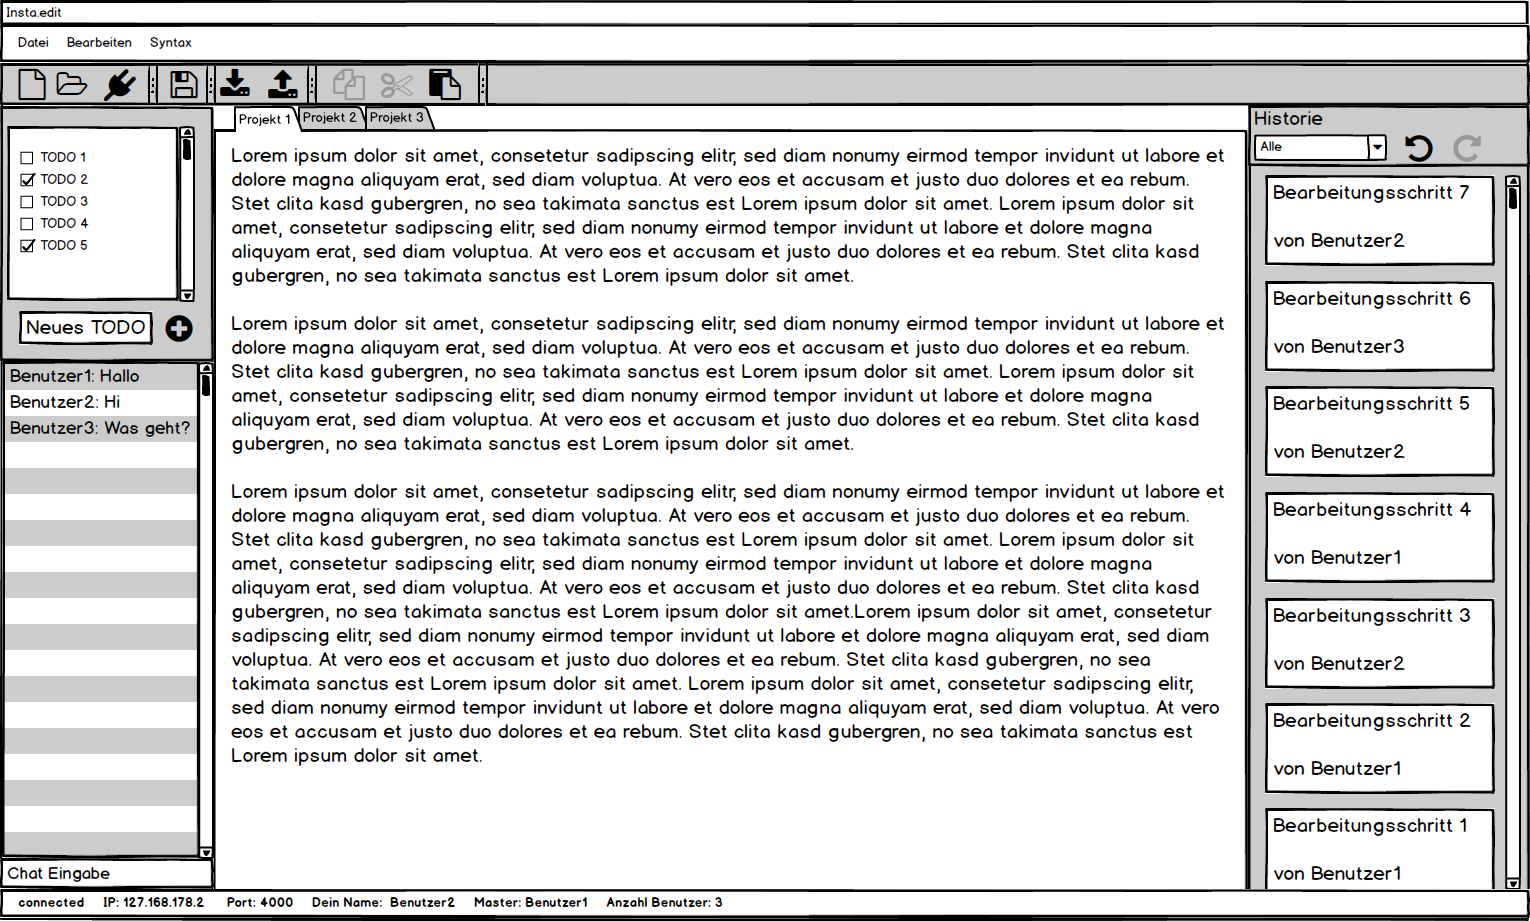
\includegraphics[width=1\textwidth]{img/screen_all}
	\label{fig:screen_all}
	\caption{So könnte die GUI während der Laufzeit aussehen.}
\end{figure}

\subsection{Allgemeines zur Benutzeroberfläche}
Der Texteditor hat eine mit Java Swing erzeugte grafischen Benutzeroberfläche, bestehend aus mehreren Komponenten. Am oberen Rand befindet sich eine Menüleiste ( \ref{subsubsec:menuleiste}), welche unabhängig von geöffneten Projekten gleich bleibt. Darunter liegen eine Toolleiste (\ref{subsubsec:toolbar}) mit Knöpfen für Funktionen und eine Tableiste (\ref{subsubsec:tableiste}) welche alle zur Zeit geöffneten Editorinstanzen anzeigt und die Möglichkeit gibt zwischen diesen zu wechseln. Eine Editorinstanz zu einem Projekt besteht aus einer Arbeitsfläche, in welcher man das Dokument bearbeiten kann (\ref{subsubsec:arbeitsflaeche}), einem Chatfenster ( \ref{subsubsec:chat}), der Bearbeitungshistorie (\ref{subsubsec:historie}), einer Infoleiste (\ref{subsubsec:info}) und einer TODO-Liste (\ref{subsubsec:todo}). Außerdem gehen für einige Funktionen Pop-Ups auf (\ref{subsubsec:popup}).

\subsection{Details zur Benutzeroberfläche}
\subsubsection{Menüleiste}
\label{subsubsec:menuleiste}
Die Menüleiste dient zur geordneten Benutzerführung und wird am oberen Rand der GUI zu finden sein. Sie ist unabhängig von der geöffneten Editorinstanz immer gleich, mit folgenden Komponenten, aufgebaut:
\begin{itemize}
\item /BO110/ Aufklapp-Menü "Datei" (Figur \ref{fig:datei}) mit Elementen :
\begin{itemize}
\item Neues Projekt* (\refFunction{f-neu})
\item Projekt öffnen* (\refFunction{f-oeffnen})
\item Mit Projekt verbinden (\refFunction{bo-verbinden})
\item Dokument importieren (\refFunction{fw-import})
\item Dokument exportieren (\refFunction{fw-exportieren})
\item Projekt speichern* (\refFunction{f-speichern})
\item Projekt speichern unter ...* (\refFunction{f-speichernUnter})
\item Projekt schließen* (\refFunction{f-closeEdit})
\item \name\ Beenden* (\refFunction{f-closeProg})
\end{itemize}

\item /BO120/ Aufklapp-Menü "Bearbeiten" (Figur: \ref{fig:bearbeiten}) mit Elementen:
\begin{itemize}
\item Lokal Rückgängig* (\refFunction{f-persUndo})
\item Lokal Wiederherstellen* (\refFunction{f-persRedo})
\item Global Rückgängig machen* (\refFunction{f-globUndo})
\item Global Wiederherstellen* (\refFunction{f-globRedo})
\item Suchen und Ersetzen* (\refFunction{bo-suchen})
\item Text kopieren* (\refFunction{f-kopieren})
\item Text ausschneiden* (\refFunction{f-ausschneiden})
\item Text einfügen* (\refFunction{f-einfuegen})
\end{itemize}
Diese Funktionen beziehen sich alle nur auf die aktuelle Editorinstanz.


\item /BOW130/ Aufklapp-Menü "Syntax"  mit Elementen:
\begin{itemize}
\item Keiner
\item Java
\item HTML
\item Python
\end{itemize}
Hierbei muss zwischen einen der vier Stilen gewählt werden (\refFunction{lw160}). Standardmäßig ist "Keiner" ausgewählt. Der ausgewählte Syntax-Stil beVerbundeneszieht sich nur auf die aktuelle Editorinstanz.
\end{itemize}

\begin{figure}[h]
	\centering
	\begin{subfigure}{.49\textwidth}
	\centering
  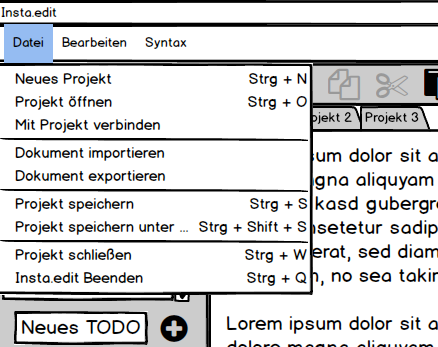
\includegraphics[width=0.85\textwidth]{img/screen_datei}
	\caption{Aufklapp-Menü "Datei"}
	\label{fig:datei}
\end{subfigure}
\begin{subfigure}{.49\textwidth}
	\centering
  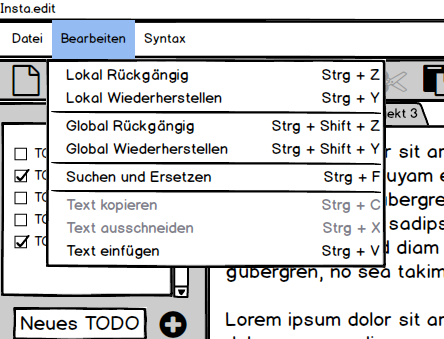
\includegraphics[width=0.85\textwidth]{img/screen_bearbeiten}\caption{Aufklapp-Menü "Bearbeiten"}
	\label{fig:bearbeiten}
	\end{subfigure}
	\caption{Menüelemente}
\end{figure}

\noindent\rule{\textwidth}{1pt}
*: Funktion wird auch über Tastenkombination aufrufbar sein (\ref{subsubsec:tastenkombinationen}).


\newpage
\subsubsection{Toolleiste}
\label{subsubsec:toolbar}

/BOW210/ Unter der Menüleiste befindet sich eine Toolbar, welche Buttons zu folgenden Funktionen hat:

\begin{itemize}
\item Neues Projekt* (\refFunction{f-neu})
\item Projekt öffnen* (\refFunction{f-oeffnen})
\item Mit Projekt verbinden (\refFunction{bo-verbinden})
\item Projekt speichern* (\refFunction{f-speichern})
\item Projekt speichern unter ...* (\refFunction{f-speichernUnter})
\item Dokument importieren (\refFunction{fw-import})
\item Dokument exportieren (\refFunction{fw-exportieren})
\item Text kopieren* (\refFunction{f-kopieren})
\item Text ausschneiden* (\refFunction{f-ausschneiden})
\item Text einfügen* (\refFunction{f-einfuegen})
\end{itemize}

Die Toolleiste wird auch unabhängig von der geöffneten Editorinstanz immer gleich angezeigt.

\noindent\rule{\textwidth}{1pt}
*: Funktion wird auch über Tastenkombination aufrufbar sein (\ref{subsubsec:tastenkombinationen}).

\subsubsection{Tableiste}
\label{subsubsec:tableiste}
/BO310/ Die Tableiste ermöglicht ein einfaches Navigieren zwischen geöffneten Editorinstanzen. Sie zeigt alle geöffneten Projekte an.

\subsubsection{Arbeitsfläche}
\label{subsubsec:arbeitsflaeche}
/BO410/ Die Arbeitsfläche bildet den zentralen Teil jeder Editorinstanz. Sie zeigt das zu bearbeitende Dokument an und erlaubt Änderungen an diesem vorzunehmen (\refFunction{f-schreiben}, \refFunction{f-loeschen}). Dabei wird ersichtlich sein, an welchen Stellen andere Benutzer aktuell Änderungen vornehmen.
Zusätzlich kann ein Benutzer über Rechtsklick auf eine ausgewählte Textstelle im Dokument Annotationen hinzuzufügen (\refFunction{f-annoHinzu}). Dies sind Kommentare, die auf dem Text im Dokument angezeigt werden und sich durch klicken  bearbeiten (\refFunction{f-annoEdit}) und wieder entfernen lassen (\refFunction{f-annoLoeschen}).
Wenn ein Syntax-Stil ausgewählt wurde (\refFunction{fw-syntax}), wird der Text in der Arbeitsfläche dementsprechend hervorgehoben. Die Arbeitsfläche beinhaltet eine Scrollbar (\refFunction{f-scrollDoc}).

\subsubsection{Chat}
\label{subsubsec:chat}
/BO510/ Das Chat-Fenster
wird aus einem Eingabefeld für neue Nachrichten und einer Fläche, die den Chatverlauf anzeigt, bestehen. 
Durch Drücken der Enter-Taste wird die getippte Nachricht an alle Benutzer des Projekts gesendet (\refFunction{f-senden}). Vor jeder Nachricht steht die jeweilige Benutzername des Senders, so dass eine übersichtliche Konversation möglich ist. Im Chatverlauf kann man scrollen (\refFunction{f-scrolChat}).

\subsubsection{Bearbeitungshistorie}
\label{subsubsec:historie}
/BO610/ Die Bearbeitungshistorie zeigt Änderungen am Dokument chronologisch an. Dabei kann ein Benutzer auswählen ob er alle Änderungen oder nur die eines bestimmten Benutzers sehen will. Außerdem gibt es hier die Möglichkeit Bearbeitungsschritte eines beliebigen Nutzers Rückgängig zu machen (\refFunction{f-persUndo}). Das Benutzerspezifische Rückgängig machen ist nur hier möglich und kann nicht über Tastenkombinationen oder Menüleisten aufgerufen werden. \\
Die Bearbeitungshistorie beinhaltet eine Scrollbar (\refFunction{f-scrolHist}).

\subsubsection{Infoleiste}
\label{subsubsec:info}
/BOW710/
In der Infoleiste werden folgende Informationen über die Editorinstanz angezeigt:
\begin{itemize}
\item Rückmeldung ob die Verbindung zum Master noch besteht
\item IP-Adresse und Port der Verbindung
\item Benutzername für die aktuelle Editorinstanz
\item Benutzername des Masters
\item Name des in der Editorinstanz geöffneten Projekts
\item Anzahl der Benutzer, welche zur Zeit aktiv am Projekt arbeiten.
\end{itemize}

\subsubsection{TODO-Liste}
\label{subsubsec:todo}
/BOW810/ 
Jedes Projekt hat eine TODO-Liste, bestehend aus einem Eingabefeld, mit dessen Hilfe man neue TODOs erstellen kann und einer Liste, in welcher die erzeugten TODOs mit Kontrollkästchen dargestellt werden. Eingegebene TODOs können per Knopfdruck oder durch Drücken der Enter-Taste zur Liste hinzugefügt werden (\refFunction{fw-todoHinzu}). Der Benutzer hat die Möglichkeit, diese TODOs abzuhaken (\refFunction{fw-todoErledigt}) oder sie zu löschen (\refFunction{fw-todoLoeschen}), nicht aber sie zu verändern. \\
Die TODO-Liste beinhaltet eine Scrollbar (\refFunction{fw-scrollTodo}).

\subsubsection{Pop-Ups}
\label{subsubsec:popup}
\begin{itemize}

\item \textbf{/BO910/ Passwort/Whitelist festlegen}
\\
Wenn ein Benutzer ein neues Projekt erstellt (\refFunction{f-neu}), ein Dokument importiert (\refFunction{fw-import}) oder ein Projekt öffnet (\refFunction{f-oeffnen}) wird der Nutzer per Pop-Up aufgefordert ein Passwort (\refFunction{f-passwort}) oder eine Whitelist (\refFunction{fw-whitelist}) für das Projekt festzulegen. Diese lassen sich während der Bearbeitung des Projekts nicht verändern. Falls das Wunschkriterium "Benutzername" erfüllt wird, muss der Benutzer sich hier auch einen Benutzernamen geben.

\item \textbf{\labelFunction{bo-verbinden}{/BO920/} Mit Projekt verbinden}
\\
Wenn ein Benutzer die "Verbinden"-Funktion (\refFunction{f-verbinde}) aufruft fragt ein Pop-Up nach der IP-Adresse und dem Port des Projektes mit dem sich der Benutzer verbinden will.

\item \textbf{/BO930/ Eingabe Passwort}
\\
Wenn ein Benutzer sich zu einem Projekt ohne Whitelist verbinden will, wird er über ein Pop-Up nach dem Passwort für das Projekt gefragt \refFunction{f-verbinde}.

\item \textbf{\labelFunction{bo-suchen}{/BO940/} Suchen und Ersetzen}
\\
Für die "Suchen und Ersetzen" Funktion öffnet sich ein Pop-Up. Dieses besteht aus zwei Textfeldern. Eins in das der Benutzer das zu suchende Wort eingeben kann und eins in das der Benutzer das ersetzende Wort eingeben kann. Weiter gibt es vier Knöpfen für "Suchen" (\refFunction{f-finden}), "Ersetzen" (\refFunction{f-ersetzen}), "Suche alle" (\refFunction{f-alleFinden}) und "Ersetze alle" (\refFunction{f-alleErsetzen}).
\end{itemize}

\subsubsection{Tastenkombinationen}
\label{subsubsec:tastenkombinationen}
/BO1010/ Für einfachere Benutzung kann man wichtige Funktionen auch durch Tastenkombinationen aufrufen. Folgende Tastenkombinationen werden im Produkt unterstützt:
\begin{itemize}
\item Neues Projekt (\refFunction{f-neu}): "Strg + N"
\item Projekt öffnen (\refFunction{f-oeffnen}): "Strg + O"
\item Projekt speichern (\refFunction{f-speichern}): "Strg + S"
\item Projekt speichern unter (\refFunction{f-speichernUnter}): "Strg + Shift + S"
\item Projekt schließen (\refFunction{f-closeEdit}): "Strg + W"
\item \name\ Beenden (\refFunction{f-closeProg}): "Strg + Q"
\item Lokal Rückgängig (\refFunction{f-persUndo}): "Strg + Z"
\item Lokal Wiederherstellen (\refFunction{f-persRedo}): "Strg + Y"
\item Global Rückgängig (\refFunction{f-globUndo}): "Strg + Shift + Z"
\item Global Wiederherstellen (\refFunction{f-globRedo}): "Strg + Shift + Y"
\item Text kopieren (\refFunction{f-kopieren}): "Strg + C"
\item Text ausschneiden (\refFunction{f-ausschneiden}): "Strg + X"
\item Text einfügen (\refFunction{f-einfuegen}): "Strg + V"
\end{itemize}
 


\section{Qualitätszielbestimmungen}
\marginpar{Florian}

Die folgenden Qualitätskriterien sollen während des Entwicklungsprozesses bzw. vom Produkt eingehalten werden.

\begin{itemize}
\item /Q100/ Plattformspezifischen Mechanismen werden nicht verwendet, um Kompatibilität und Portabilität sicherzustellen.
\item /Q110/ Die Verwendung von Javadoc wird den Quellcode übersichtlich und verständlicher machen.
\item /Q120/ Durch Verwendung des Model-View-Controller-Patterns wird eine geringe Kopplung zwischen den einzelnen Programmteilen erreicht.
\item /Q130/ Durch Verschlüsselung des Netzwerkverkehrs wird die Vertraulichkeit der Daten sichergestellt.
\item /Q140/ Eine einfache Bedienbarkeit wird durch eine übersichtliche Menüleiste und Tastaturkürzel für wichtige Funktionen ermöglicht.
\end{itemize}

\section{Entwicklungsumgebung}
\marginpar{Pascal}
Die Umgebung wird beschrieben, in der das zu erstellende Produkt entwickelt wird. \\ \\
Für die reine Software-Entwicklung werden folgende Tools verwendet. 

\begin{itemize}
\item IntelliJ Community (2017.2.5) und Eclipse (4.7) zum Entwickeln der Java-Dateien.
\item JUnit (Version 5) zum Validieren
\item IBM Rational Software Architect (Version 8.0 oder höher) für Entwurf und Modellierung
\end{itemize}
Sonstige Tools werden für Dokumentation und Kommunikation verwendet:
\begin{itemize}
\item Gitkraken als git client für die Versionskontrolle
\item gitlab.com als Host des git repositories
\item \LaTeX\ zum Erstellen von Dokumenten
\item Slack zur Kommunikation und zum Austausch von Protokollen der Teamtreffen sowie erstellten PDF-Dokumenten
\item E-Mail-Clients (u.a. Thunderbird) zur Kommunikation
\item Chrome, Firefox und Internet Explorer als Web Browser
\item Balsamiq als Tool zum Erstellen von Mockups der GUI
\item Sublime Text 3, nano und atom als Texteditoren
\end{itemize}

\section{Testszenarien und Testfälle}
\marginpar{Cedric}

Hier werden alle Tests aus Anwendersicht aufgeführt, die bei der Abnahme des Software-Produkts durchlaufen werden müssen. Jede relevante Produktfunktionen wird durch die entsprechenden Testfälle abgedeckt. Jede Funktion wird separat getestet.
Innerhalb jeder Testgruppe bauen die einzelnen Tests aufeinander auf. Dies hat zur Folge, dass die Tests unbedingt in der angegebenen Reihenfolge durchgeführt werden müssen. Ist das nicht der Fall, ist es klar gekennzeichnet.

\subsection{Testdaten}
\begin{itemize}
\item Benutzer:
\begin{itemize}
\item Benutzer 1:
\begin{itemize}
\item Benutzername : Benutzer1
\end{itemize} 
\item Benutzer 2
\begin{itemize}
\item Benutzername : Benutzer2
\end{itemize} 
\item Benutzer 3
\begin{itemize}
\item Benutzername : Benutzer3
\end{itemize}
\item Falls ein Benutzer Master ist, ist sein Benutzername "Master". 
\end{itemize}
\item Textdatei: 
\begin{itemize}
\item TestTextdatei.txt
\end{itemize}
\item Projektdateien
\begin{itemize}
\item TestProjekt.json
\item LastTest.json
\end{itemize}
\end{itemize}

\subsection{Tests zum Erstellen eines Dokumentes}
\begin{itemize}
\item{\labelFunction{t200} {/T200/}}
Benutzer1 startet das Programm zum ersten Mal. Die GUI wird korrekt dargestellt.
\item{\labelFunction{t210} {/T210/}}
Test zu \refFunction{f-neu} 
\\
Benutzer1 klickt auf "Datei" und wählt "Neues Projekt". Die Wahlmöglichkeit zwischen Passwort und Whitelist wird korrekt dargestellt. Benutzer1 wählt die Option Passwort. Das Eingabefeld des Passworts wird korrekt dargestellt. Benutzer1 gibt das Passwort "passwort" ein. Ein leeres Dokument wird dargestellt, außerdem wird der Port "40000", die IP-Adresse "10.0.0.1", und der Benutzername des Masters, in diesem Falle der Eigene, "Master", in der Statusleiste angezeigt.

\item{\labelFunction{t220} {/T220/}}
Test zu \refFunction{f-oeffnen}
\\
Benutzer1 klickt auf "Datei" und wählt "Projekt Öffnen". Benutzer1 wählt die Option Passwort und gibt das Passwort "passwort1" ein. Der Auswahldialog wird korrekt dargestellt. Benutzer1 wählt "TestProjekt.json" aus dem Ordner "\textasciitilde{}/TestDirectory". Das Dokument wird in einer neuen Editorinstanz korrekt dargestellt. 


\item{\labelFunction{tw230} {/TW230/}}
Test zu \refFunction{fw-import}
\\
Benutzer1 klickt auf Datei und wählt "Text Importieren". Benutzer1 wählt die Option Passwort und gibt das Passworts "passwort1" ein. Der Auswahldialog wird korrekt dargestellt. Benutzer1 wählt "TestTextdatei.txt" aus dem Ordner 
"\textasciitilde{}/TestDirectory". Der Text wird in einer neuen Editorinstanz korrekt dargestellt, außerdem werden die restlichen Komponenten der GUI (Historie, Statusleiste) korrekt dargestellt.


\item{\labelFunction{tw240} {/TW240/}}
Test zu \refFunction{f-neu}  und \refFunction{fw-whitelist}
\\
Benutzer1 klickt auf "Datei" und wählt "Neues Projekt". Die Wahlmöglichkeit zwischen Passwort und Whitelist wird korrekt dargestellt. Benutzer1 wählt die Option Whitelist. Das Feld zum Eintragen der zugelassenen IP-Adressen wird korrekt dargestellt. Er fügt die IP-Adressen "10.0.0.4" und "10.0.0.5" zu den erlaubten IP-Adressen hinzu. Das Dokument wird in einer neuen Editorinstanz korrekt dargestellt.
\end{itemize}


\subsection{Tests zum Verbinden mit einem Dokument}
Tests zu \refFunction{f-verbinde}
\\Der erste Test wird im Zustand nach Test \refFunction{t210} durchgeführt.
\begin{itemize}
\item{\labelFunction{t300} {/T300/}}
Benutzer2 klickt auf "Datei" und wählt "Verbinde". Die Abfrage von IP-Adresse und Port wird korrekt dargestellt.
\item{\labelFunction{t305} {/T305/}}
Benutzer2 gibt eine falsche IP-Adresse "10.0.0.19" ein und den richtigen Port "40000". Eine Fehlernachricht wird angezeigt.
\item{\labelFunction{t310} {/T310/}}
Benutzer2 gibt die richtige IP-Adresse "10.0.0.1" ein und den falschen Port "40002" ein. Eine Fehlernachricht wird angezeigt.
\item{\labelFunction{t315} {/T315/}}
Benutzer2 gibt die richtige IP-Adresse "10.0.0.1" ein und den richtigen Port "40000". 
Die Passwortabfrage wird korrekt dargestellt.
\item{\labelFunction{t320} {/T320/}}
Benutzer2 gibt das falsche Passwort "falsch" ein. Die Fehlernachricht wird korrekt dargestellt. Dies wird drei mal wiederholt.
Nach dem dritten Fehlversuch wird die Verbindung zu Benutzer1 abgebrochen. Die Fehlermeldung wird korrekt dargestellt.
\item{\labelFunction{t325} {/T325/}}
Benutzer2 versucht sich mit dem Dokument von Benutzer1 zu verbinden. Nach Eingabe der richtigen IP-Adresse "10.0.0.1" und dem richtigen Port "40000" wird die Passwortabfrage korrekt dargestellt.
Er gibt das richtige Passwort "passwort" ein.
Das Dokument wird korrekt dargestellt.
\end{itemize}
Es wird ein neues Testszenario gestartet.\\
Dieses testiert immer noch \refFunction{f-verbinde}.\\
Der erste Test wird im Zustand nach Test \refFunction{tw240} durchgeführt.

\begin{itemize}
\item{\labelFunction{tw330} {/TW330/}}
Benutzer2 benutzt in diesem Fall die IP-Adresse "10.0.0.3" im LAN-Netzwerk.
Benutzer2 klickt auf "Datei" und wählt "Verbinde".
Benutzer2 versucht sich mit dem Dokument von Benutzer1 zu verbinden. Nach Eingabe der richtigen IP-Adresse "10.0.0.1" und dem richtigen Port "40000" wird die Abfrage des Benutzernamens korrekt dargestellt.
\item{\labelFunction{t335} {/TW335/}}
Benutzer2 gibt den Benutzernamen "Master" ein.
Da dieser Benutzername schon vergeben ist erscheint eine Fehlermeldung.
Eine Fehlermeldung wird korrekt dargestellt.
\item{\labelFunction{tw340} {/TW340/}}
Benutzer2 gibt den Benutzernamen "Benutzer2" ein.
Das Dokument wird korrekt dargestellt.
\end{itemize}


\subsection{Tests zum Editieren eines Dokumentes}
Der erste Test wird im Zustand nach Test \refFunction{t210} durchgeführt.
\begin{itemize}
\item{\labelFunction{t405} {/T405/}}
Test zu \refFunction{f-schreiben} und \refFunction{f-loeschen}\\
Benutzer1 fügt durch tippen den Text "Hello !" in das Dokument ein.  Der Text wird korrekt dargestellt. Er löscht den gerade geschriebenen Text. Dies wird korrekt dargestellt. 
Benutzer1 fügt durch Tippen den Text "Hello World !" in das Dokument ein. 
\item{\labelFunction{t410} {/T410/}}
Test zu \refFunction{f-finden}\\
Durch das Tippen von "Strg+F" erscheint ein Pop-Up mit der Möglichkeit den Text zu durchsuchen. Er sucht nach "Hel". Der gesuchte Text wird markiert. 
Benutzer1 sucht nach "xyz", ein Fehlermeldung wird angezeigt.

\item{\labelFunction{t415} {/T415/}}
Test zu \refFunction{f-ersetzen}\\
Benutzer1 sucht nach "h" und fügt "t" in das Feld "Ersetzen" ein. Benutzer1 klickt auf "Ersetzen" Die Änderungen werden korrekt angezeigt.
\item{\labelFunction{t420} {/T420/}}
Test zu \refFunction{f-alleErsetzen}
Test zu \refFunction{f-alleFinden}\\
Benutzer1 fügt "ll" ans Ende des Dokumentes an.
Benutzer1fügt "ll" in das Feld "Alle Finden" ein und führt "xx" in das Feld "Ersetze alle" ein. Benutzer1 klickt auf "Ersetze alle".Die Änderungen werden korrekt dargestellt.
\item{\labelFunction{t425} {/T425/}}
Test zu \refFunction{f-kopieren}
Test zu \refFunction{f-einfuegen}
Test zu \refFunction{f-ausschneiden}\\
Benutzer1 selektiert "Hexxo" und fügt es in die Zwischeneingabe durch "Strg+C" ein.  Benutzer1 fügt den in der Zwischeneingabe gespeicherten Text an der Stelle des Cursors durch das Tippen von "Strg+V" ein. Der Text "texxo"wird korrekt dargestellt.
Benutzer1 selektiert "texxotexxo" und fügt es in die Zwischeneingabe durch "Strg+x" ein. Der Text wird korrekt entfernt. 
Benutzer1 fügt den in der Zwischeneingabe gespeicherten Text an der Stelle des Cursors durch das Tippen von "Strg+V" ein. Der Text "texxo"wird korrekt dargestellt.
\item{\labelFunction{t430} {/T430/}}
Benutzer2 verbindet sich mit dem Dokument von Benutzer1, wie in \refFunction{t325}.
Benutzer2 fügt einen Satz "Hello Master" durch Tasteneingabe in seiner Editorinstanz hinzu. 
Die Änderung wird bei Benutzer1 korrekt dargestellt.
\item{\labelFunction{t435} {/T435/}}
Test zu \refFunction{f-annoHinzu}\\
Benutzer 1 bewegt den Cursor an die erste Stelle der ersten Zeile. Dort tätigt er einen Rechtsklick und wählt "Annotation Hinzufügen". Im nun angezeigten Feld schreibt Benutzer1 "Dies ist eine Annotation".
Dies wir korrekt dargestellt.
Außerdem wird Benutzer2 die Annotation korrekt dargestellt.
\item{\labelFunction{t440} {/T440/}}
Test zu \refFunction{f-annoEdit} und \refFunction{f-annoLoeschen}
\\
Benutzer2 klickt auf die Annotation in Zeile 1. Die Annotation wird korrekt dargestellt. 
Benutzer2 fügt der Annotation den Text "Seen" hinzu. Dies wird korrekt dargestellt. Benutzer2 klickt auf das Kreuz der Annotation. Diese verschwindet und ist somit gelöscht. Dies wird bei allen Benutzern korrekt dargestellt.
\item{\labelFunction{t445} {/T445/}}
Tests zu \refFunction{f-persUndo},\refFunction{f-persRedo}, \refFunction{f-globUndo} und \refFunction{f-globRedo}\\
Benutzer3 verbindet sich mit dem Dokument von Benutzer1, wie in \refFunction{t325}.
Benutzer3 fügt das Wort "test" an Ende des Dokumentes hinzu.
Benutzer2 klickt auf die Liste der Benutzer über der Historie.
Dort wählt er Benutzer3 aus.
Benutzer2 nutzt die  Undo-Funktion. Der letzte Schritt von Benutzer3 wird korrekt aufgehoben das Wort "test" am Ende des Dokumentes wird gelöscht.
Benutzer2 nutzt die Nutzerspezifische(Benutzer3) Redo-Funktion. Das vorherige Undo von Benutzer3 wird aufgehoben.
Benutzer1 nutzt die globale Undo-Funktion. Der letzte Schritt wird korrekt aufgehoben.
Benutzer2 nutzt die globale Redo-Funktion. Der letzte Schritt wird korrekt aufgehoben.
\item{\labelFunction{t450} {/T450/}}
Die Latenz zwischen Benutzer1 und Benutzer2 liegt bei 100ms. 
Die Latenz zwischen Benutzer1 und Benutzer3 liegt bei 200ms.
Benutzer2 fügt am Anfang des Dokumentes "a" hinzu. 
Bevor diese Änderung bei Benutzer 3 angekommen ist fügt dieser ein "b" am Anfang des Dokumentes ein. 
Es wird korrekt bei allen Benutzern das "a" von Benutzer2 hinzugefügt.
Da beide auf der gleichen Version eine Änderung eingeführt haben wird nur die erste, in diesem Falle die von Benutzer2, angenommen.
\item{\labelFunction{tw455} {/TW455/}}
Benutzer2 löscht den ganzen Text. 
Benutzer3 schreibt "abc"
Benutzer2 fügt ein "a" zwischen "a" und "b" von "abc". 
Benutzer3 fügt ein "d" zwischen "a" und "b" von "abc".
Die Änderung von Benutzer2 kommt als erste beim Server an.
Bei Benutzer1, Benutzer2 und Benutzer3 wird korrekt "aadbc" dargestellt.
\end{itemize}


\subsection{Tests zum Speichern/Schließen eines Dokumentes}
Diese Tests werden im Zustand nach den Tests \refFunction{t210} und \refFunction{t305} ausgeführt.

\begin{itemize}
\item{\labelFunction{t500} {/T500/}}
Test zu \refFunction{f-speichernUnter}\\
Benutzer1 klickt auf "Datei" und wählt "Projekt Speichern Unter". Der Auswahldialog wird korrekt dargestellt. Benutzer1 wählt den Ordner "\textasciitilde{}/testDirectory" aus. Er nennt das Projekt "test5.json". Die Datei wird korrekt gespeichert.
\item{\labelFunction{t510} {/T510/}}
Test zu \refFunction{fw-exportieren}\\
Benutzer1 klickt auf "Datei" und wählt "Projekt Exportieren". Der Auswahldialog wird korrekt dargestellt. Benutzer1 wählt den Ordner "\textasciitilde{}/testDirectory" aus. Er nennt die Datei "test6.txt". Die Datei wird korrekt gespeichert.
\item{\labelFunction{t520} {/T520/}}
Test zu \refFunction{f-closeEdit}\\
Benutzer1 erstellt ein neues Projekt nach dem Verfahren in \refFunction{t210}. 
Benutzer1 schreibt "Hello World !" in das Dokument. 
Benutzer1 schliesst die Editorinstanz. 
Das Pop Up, welches den Nutzer fragt ob er die ungesicherten Änderungen speichern möchte, wird korrekt dargestellt.
\item{\labelFunction{t530} {/T530/}}
Test zu \refFunction{f-closeProg}\\
Benutzer1 erstellt zwei neue Projekte nach dem Verfahren in \refFunction{t210}. 
Benutzer1 schreibt "Hello World !" in die Dokumente.
Benutzer1 schließt das Programm. 
Das Pop Up zum Speichern der Dokumente wird korrekt dargestellt.
\end{itemize}
Der Test \refFunction{t325} wird ausgeführt.
\begin{itemize}
\item{\labelFunction{t540} {/T540/}}
Der Test \refFunction{t520} wird durch den Benutzer2 durchgeführt.
\item{\labelFunction{t550} {/T550/}}
Benutzer1 klickt auf Datei und wählt "Text Exportieren". Der Auswahldialog wird korrekt dargestellt. Der Benutzer wählt den Ordner "\textasciitilde{}/testDirectory" und gibt dem Dokument den Namen "test7.txt".
\item{\labelFunction{t560} {/T560/}}
Der Test \refFunction{t550} wird durch Benutzer2 durchgeführt. 
\end{itemize}

\subsection{Tests zum Umgang von Verbindungsverlust zum Master}
Diese Tests werden im Zustand nach den Tests \refFunction{t210} und \refFunction{t325}ausgeführt.
Sie werden alle einzeln durchgeführt. Dies heißt das sie nicht voneinander abhängen.
\begin{itemize}
\item{\labelFunction{t600} {/T600/}}
Benutzer1 schließt seine Programinstanz. Benutzer2 wird die korrekte Meldung angezeigt, das sein Master nicht mehr verbunden ist. Er kann lokal weiter den Text editieren. 
\item{\labelFunction{t610} {/T610/}}
Benutzer1 bricht seine LAN-Verbindung ab. 
Benutzer2 wird korrekt benarichtigt. Benutzer2 gibt "Hello World" in den Editor ein.
Benutzer1 verbindet sich erneut (die Verbindung wird in mehr als 10 Sekunden wieder hergestellt). 
Benutzer2 wird nicht benachrichtigt, und ist nicht mehr mit dem Projekt von Benutzer1 verbunden.
\item{\labelFunction{t620} {/T620/}}
Benutzer3 verbindet sich mit dem gleichen Verfahren wie in \refFunction{t325} zu dem Dokument von Benutzer1. 
Benutzer1 bricht seine LAN-Verbindung ab. 
Benutzer2 wird korrekt benachrichtigt. Benutzer2 gibt "Hello World" in den Editor ein.
Benutzer3 wird korrekt benachrichtigt. Benutzer3 gibt "Hey you !" in den Editor ein. 
Benutzer1 baut seine LAN-Verbindung erneut auf.
Die Editorinstanz von Benutzer1 verbindet sich automatisch erneut (dies passiert innerhalb von 10 Sekunden). 
Die Änderungen am Dokument werden bei Benutzer1, Benutzer2 und Benutzer3 korrekt dargestellt. 
\end{itemize}

\pagebreak

\subsection{Tests zum Chat}
Tests zu \refFunction{f-senden}\\
Diese Tests werden im Zustand nach den Tests \refFunction{t210} und \refFunction{t325}ausgeführt.
\begin{itemize}
\item{\labelFunction{t700} {/T700/}}
Benutzer1  Sendet "Hey" im Chat. Die Nachricht wird im eigenem und im Chat von Benutzer2 korrekt angezeigt.
\item{\labelFunction{t710} {/T710/}}
Benutzer3 verbindet sich nach dem Vorgehen in \refFunction{t325}.
Benutzer1 sendet "Hey". 
Die Nachricht wird bei allen Benutzern korrekt dargestellt.
Benutzer2 sendet "Hey Back". 
Die Nachricht wird bei allen Benutzern korrekt dargestellt.
Benutzer2 sendet "Benutzer3 are you on?".
Die Nachricht wird bei allen Benutzern korrekt dargestellt.
Benutzer3 sendet "Yes!". 
Die Nachricht wird bei allen Benutzern korrekt dargestellt.

\end{itemize}

\subsection{Tests zur TODO-Liste}
Der erste Test wird im Zustand nach den Tests \refFunction{t210} und \refFunction{t325} durchgeführten Tests ausgeführt.
\begin{itemize}
\item{\labelFunction{tw800} {/TW800/}}
Test zu \refFunction{fw-todoHinzu}\\
Benutzer1 fügt den Text "Test TODO" in das Feld "Neues TODO", dann klickt er auf das "+". Das neue TODO wird bei allen Nutzern korrekt dargestellt.
\item{\labelFunction{tw810} {/TW810/}}
Test zu \refFunction{fw-todoErledigt}\\
Benutzer2 klickt die CheckBox bei "Test TODO". Die Änderung wird bei allen Nutzern korrekt dargestellt.
\item{\labelFunction{tw820} {/TW820/}}
Test zu \refFunction{fw-todoLoeschen}\\
Benutzer1 klickt auf das Kreuz um das "Test TODO" zu löschen. 
Der Eintrag in der TODO Liste verschwindet bei allen Benutzern. 
\end{itemize}

\subsection{Lasttests}
\begin{itemize}
\item{\labelFunction{tw900} {/T900/}}
Benutzer1 erstellt nach dem Verfahren des Test \refFunction{t210} mit der Datei "LastTest.json" ein Dokument.
Benutzer2 verbindet sich nach dem Verfahren des Tests \refFunction{t325}. Nach dem Bestätigen des Benutzernamens wird die Datei in 15 Sekunden geladen. 
\item{\labelFunction{tw900} {/T900/}}
Benutzer1 erstellt nach dem Verfahren des Tests \refFunction{t210} 10 Projekte. 
Zu jedem Projekt verbinden sich 10 verschiedene Benutzer.
Die Bearbeitung der Dokumente funktioniert ohne spürbare Verzögerung.
\end{itemize}
%TODO loeschen annoloeschen 


\clearpage
%Wird hier gebraucht, da ansonsten das Bild erst auf einer anderen Seite gezeichnet wird.
\section{Systemarchitektur}
\marginpar{Pascal}

Die Architektur wird grob durch Grafik \ref{fig:architektur} dargestellt:

\begin{figure}[h]
	\centering
    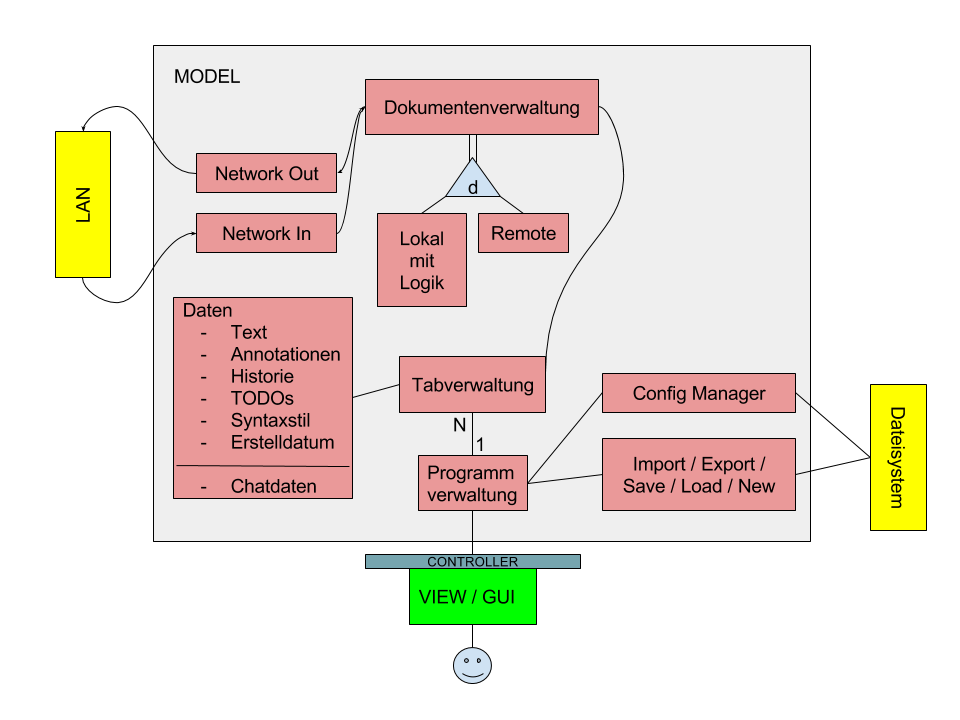
\includegraphics[width=0.9\textwidth]{img/architektur}
    \caption{Grafik zur Illustration der groben Architektur}
	\label{fig:architektur}
\end{figure}

Im Folgenden werden die Aufgaben der einzelnen Bestandteile des Diagramms erklärt. \\ Pfade ohne Beschriftung repräsentieren eine bidirektionale Verbindung, d.h. beide Komponenten kommunizieren miteinander. 1:1-Funktionalitäten werden aus Gründen der Übersichtlichkeit weggelassen. Eine 1:1-Beziehung bedeutet, dass genau eine Instanz einer Komponente mit genau einer anderen Instanz kommuniziert.
Analog bedeutet eine 1:N-Beziehung, dass eine Instanz der Komponente mit N Instanzen einer anderen Komponente kommuniziert.
\\

\begin{itemize}
\item Smiley: Der Benutzer des Programms.

\item GUI: Benutzeroberfläche, die dem Benutzer angezeigt wird und Ein-/Ausgaben verwaltet.
\item Controller: Programmeinheit, welche auf die Aktionen (Klicks mit der Maus und Tastatureingaben) des Benutzers entsprechend reagiert.

\item Dokumentenverwaltung: Programmbaustein der für Zugriffsrechte und Konfliktauflösung eines Dokuments zuständig ist. Die Dokumentenverwaltung ist eine abstrakte Klasse, welche weiter in Lokal und Remote spezialisiert wird.

\begin{itemize}
\item Lokale Dokumentenverwaltung: Die Funktionalität der Dokumentenverwaltung wird lokal erbracht.
\item Remote Dokumentenverwaltung: Die Funktionalität wird über das Netzwerk an die lokale Dokumentenverwaltung delegiert und dort erbracht.
\end{itemize}

\item Tabverwaltung: Verantwortliche Verwaltungseinheit, welche mit einer geöffneten Editorinstanz, welche ein Projekt beinhaltet, verknüpft ist und die jeweiligen Daten des Projekts beinhaltet.

\item Programmverwaltung: Verwaltungseinheit, die die ganze geöffnete Programminstanz verwaltet und steuert.

\item Daten: Die Daten des aktuell geöffneten Projekts.
\item Config Manager: Programmeinheit, welche die gewählte Fenstergröße und das Verhältnis der Komponenten der GUI in einer Config-Datei persistiert.

\item Import/Export/Save/Load/New: Programmeinheit, welche Dokumente und Projekte vom Dateisystem lädt und speichert.

\item Dateisystem: Das Dateisystem, welches vom Betriebssystem des Anwenders bereit-gestellt wird.
\item Network Out/In: Die Programmeinheit, die die lokale Netzwerkkommunikation mit anderen Benutzern des Texteditors sicher stellt.
\item LAN: Die physikalische Umsetzung der Kommunikation über das Ethernet-Netzwerkkabel.
\end{itemize}


\section{Systemevolution}
\marginpar{Florian}
Folgende Erweiterungen und Verbesserungen sind im Zuge der Systemevolution denkbar:

\begin{itemize}
\item Die graphische Benutzeroberfläche kann umgestaltet werden, falls sich ein anderes Layout als übersichtlicher herausstellt.
\item Die graphische Benutzeroberfläche kann auch durch eine andere Schnittstelle ausgetauscht werden, zum Beispiel durch zusätzliche Steuerung über die Kommandozeile für bestimmte Operationen.
\item Längere Netzwerkausfälle (länger als 10s) könnten durch eine Verbesserung der Pufferungsmechanismen überbrückt werden.
\item Das Format der Projektdatei kann geändert werden, falls eine kompaktere Speicherungsmöglichkeit gefunden wird oder neue Features hinzukommen.
\item Es kann eine Unterstützung für Rich Text (verschiedene Schriftarten, Schriftgröße etc.) hinzugefügt werden.
\item Eine Erweiterung der Unterstützung für Syntaxstile ist möglich.
\item Den Annotationen im Text könnte eine Kommentarfunktion hinzugefügt werden.
\item Es kann eine Schnittstelle für die Erweiterung durch Plugins hinzugefügt werden.
\end{itemize}

\newpage

\section{Glossar}
\marginpar{Klara}

\newcolumntype{b}{X}
\newcolumntype{s}{>{\hsize=.5\hsize}X}

  \begin{tabularx}{\linewidth}{
    >{\hsize=.7\hsize}X|% 35% of 2\hsize 
    >{\hsize=1.3\hsize}X% 65% of 2\hsize
       % sum=2.0\hsize for 2 columns
  }

\hline
\textbf{Änderungsdatensatz} & Ein Eintrag in der Historie, also alle Daten zu einer Änderung, die am Dokument gemacht wurde. \\ \hline

\textbf{Annotation} & Eine Anmerkung im Dokument, die zusätzlich zum Text besteht. Sie ist für alle Nutzer sichtbar. \\ \hline

\textbf{Auswahldialog} & Ein Pop-Up-Fenster, in dem der Benutzer eine Datei auf seinem Computer auswählen kann. \\ \hline

\textbf{Benutzername} & Ein Benutzername muss mindestens ein Zeichen lang sein, darf höchstens zwanzig Zeichen lang sein und kann aus Groß-, Kleinbuchstaben und Zahlen bestehen. Er wird im Projekt für die Verwaltung der Änderungen und die Anzeige der Historie und des Chats verwendet. \\ \hline

\textbf{Client} & Die Editorinstanz, welche mit einem Master verbunden ist, um ein Dokument zu bearbeiten. \\ \hline

\textbf{Dokument} & Als Teil des Projekts das reine Textdokument, an dem mit \name\ gearbeitet werden kann. \\ \hline

\textbf{Editorinstanz} & Ein Tab innerhalb einer Produktinstanz. Eine Editorinstanz verwaltet ein Projekt und kann entweder als Master oder als Client agieren. \\ \hline

\textbf{GUI}  & Graphical User Interface. Die grafische Benutzeroberfläche, über die sich das Programm bedienen lässt. \\ \hline

\textbf{Installation} & Eine Programmroutine, die vor dem ersten Ausführen notwendig ist. Sie kopiert alle nötigen Programmdateien auf den Computer und konfiguriert sie so, dass das Programm zur Ausführung bereit ist \\ \hline

\textbf{IPv4} & Internet Protocol Version 4. Ein Protokoll, das Datenpakete im Internet adressiert, sodass sie an der richtigen Stelle ankommen, und der De-facto-Standard ist. \\ \hline

\textbf{IPv6} & Internet Protocol Version 6. Die nächste Version des IPv4, die die selbe Funktion übernimmt, aber noch nicht so weit verbreitet ist. \\ \hline

\textbf{Kontrollkästchen} & Ein klickbares Kästchen, das zur Anzeige von ja/nein-Werten dient. Ist das Kästchen ausgewählt (zeigt es ja an), kann es durch anklicken deselektiert werden und umgekehrt. \\ \hline

\textbf{LAN} & Local Area Network. Die lokale Netzwerkverbindung des Rechners, beispielsweise über Ethernet, über die mit anderen Endgeräten im gleichen LAN kommuniziert wird. \\ \hline

\textbf{Master} & Die Editorinstanz, die die Freigabe des Dokuments an andere Editorinstanzen verwaltet und Änderungen aller bearbeitenden Editorinstanzen zusammenführt. \\ \hline

\textbf{Produkt} & Das Programm, das auf Basis dieses Pflichtenhefts ent-wickelt wird. \\

\end{tabularx}

  \begin{tabularx}{\linewidth}{
    >{\hsize=.7\hsize}X|% 35% of 2\hsize 
    >{\hsize=1.3\hsize}X% 65% of 2\hsize
       % sum=2.0\hsize for 2 columns
  }
\hline

\textbf{Produktinstanz} & Eine Instanz des Programms, die auf einem Endgerät läuft. \\ \hline

\textbf{Projekt} & Ein Projekt umfasst das Dokument selbst und alle Teile, die mit dem Dokument in Verbindung stehen, also die Historie, den Chat, die TODO-Liste und die Annotationen. \\ \hline

\textbf{RTT} & Round Trip Time. Die Zeit die ein Paket im Netzwerk benötigt, um von einem Rechner zu einem anderen und wieder zurück gesendet zu werden. \\ \hline

\textbf{Speicherortdialog} & Ein Pop-Up-Fenster, das beim Speichern einer Datei benötigt wird. Der Benutzer kann einen Ordner auf seinem Endgerät auswählen, um die Datei dort zu speichern, und außerdem einen Namen und ein Format für die Datei festlegen. \\ \hline

\textbf{TCP} & Transmission Control Protocol. Ein Transportprotokoll, das über IPv4 und IPv6 hinaus weitere Funktionen zur Verfügung stellt. TCP ist der De-facto-Standard bei Transportprotokollen. \\ \hline

\end{tabularx}

\end{document}